%!TEX root = ../thesis.tex
\chapter{State of the art} \label{chap:sota}

\section*{}

Neste capítulo é feita uma revisão bibliográfica e descrito o estado da arte do \emph{software} de localização de falhas, como o \emph{Barinel}, das diferentes abordagens de predição de defeitos e ainda de \emph{Software Repository Mining}.

%!TEX root = ../thesis.tex
\section{Fault Localization Software}

Fault Localization Software helps to automatically locate code that generates faults when it is executed, reducing the costs associated with finding it, which would have to be done manually by the developer.  There are three main types of approach: \emph{Program Slicing}, \emph{Spectrum-based diagnosis} and \emph{Model-based diagnosis}. The \emph{Spectrum-based diagnosis} approaches will have a more detailed analysis due to their greater relevance to this work.

% 
% ==========
% Program Slicing
% ==========
%

\subsection{\emph{Program Slicing}}

Introduced by Mark Weiser in 1981 \cite{Weiser1981, Weiser1982}, this method starts its analysis from the fault and, by way of the program's data and control flow, tries to find where the problem originates. 

By removing all statements that won't affect the data set or program flow, this method determines a section of code (slice) corresponding to all statements that may be the root of the problem and must be inspected. \cite{Perez2004}. By reducing the amount of statements that require inspection, the time needed to fix an error is also reduced.

Usually, a static analysis of the program will result in a huge section of code, so there are other, dynamic, methods that will considerably reduce its size, such as \emph{program dice} or \emph{dynamic program slicing} \cite{Perez2004}.

% 
% ==========
% Spectrum-based diagnosis
% ==========
%

\subsection{\emph{Spectrum-based diagnosis}}

\emph{Spectrum-based Fault Localization} (SFL) is a probability-based fault detection method that will estimate each software component's probability of containing faults by analyzing execution-related information, whether that execution is successful or not \cite{Abreu2007}. This method is able to generate good results when the project contains a big amount of test cases and can be executed swiftly, being able to scale well to big projects \cite{Mayer2008}.

This method generates a matrix based of data saved during the execution (\emph{program spectrum} \cite{Reps1997}), connecting each test case ran with the components executed and the result, successful or unsuccessful, of that test.

\begin{table}[H]
  \centering
  \begin{tabular}{c|ccc|c} 
    & \multicolumn{3}{c|}{\textit{obs}} &  \\
    & $c_1$ & $c_2$ & $c_3$ & e \\ 
    \hline
    $t_1$ & 1 & 1 & 0 & 1 \\
    $t_2$ & 0 & 1 & 1 & 1 \\
    $t_3$ & 1 & 0 & 0 & 1 \\
    $t_4$ & 1 & 0 & 1 & 0 \\
  \end{tabular}
  \caption{\emph{Hit-spectra matrix}}
  \label{tab:hit-spectra}
\end{table}

With this matrix, also called \emph{hit-spectra matrix}, a \emph{similarity coefficient} is calculated for each of the components \cite{Abreu2009}, showing how likely it is that a component may have a fault. The way this coefficient is calculated is different, depending on the algorithm used. For example, \emph{Pinpoint} \cite{Chen2002}, \emph{Tarantula} \cite{Jones2005} and \emph{Ochiai} \cite{Abreu2007}, each, respectively, calculate the coefficient as follows
%
\begin{equation}
  s_J(j) = \frac {a_{11}(j)} {a_{11}(j) + a_{01}(j) + a_{10}(j)}
\end{equation}
%
\begin{equation}
  s_T(j) = \frac  { \frac {a_{11}(j)} {a_{11}(j) + a_{01}(j)} } 
          { \frac{a_{11}(j)}{a_{11}(j) + a_{01}(j)} + \frac{a_{10}(j)}{a_{10}(j) + a_{00}(j)}}
\end{equation}
%
\begin{equation}
  s_O(j) = \frac  {a_{11}(j)} 
          {\sqrt{(a_{11}(j) + a_{01}(j)) * (a_{11}(j) + a_{10}(j))}}
\end{equation}


% 
% ==========
% Model-based diagnosis
% ==========
%

\subsection{\emph{Model-based diagnosis}}

The basis of \emph{Model-based diagnosis} is comparing the model, i.e. the description of the system's behavior, with the actually observed behavior \cite{Mayer2008}. The difference between the two is then used to identify components that may explain errors occurred. This actually requires a formal description of the system,  which makes the task harder \cite{Perez2004}.

In order to facilitate using this method, the model is usually inferred by using the software itself, specifically, by using the test cases defined in it \cite{Perez2004}.

Although this method generates high-reliability results, the computational effort required to create a model for a big program will prevent it to be used in real projects most of the times \cite{Mayer2008}.

% 
% ==========
% Barinel
% ==========
%

\subsection{Barinel}

Barinel is an algorithm inspired by the two methods previously described, \emph{program-spectra based} and \emph{model-based diagnosis}, thus being able to generate better results than the other approaches, albeit with a slightly higher cost \cite{Abreu2009}.

This algorithm starts by analyzing a \emph{hit-spectra matrix}, representing a connection between the executed tests, the executed components, and their final result.

\begin{table}[H]
  \centering
  \begin{tabular}{c|ccc|c} 
    & \multicolumn{3}{c|}{\textit{obs}} &  \\
    & $c_1$ & $c_2$ & $c_3$ & e \\ 
    \hline
    $t_1$ & 1 & 1 & 0 & 1 \\
    $t_2$ & 0 & 1 & 1 & 1 \\
    $t_3$ & 1 & 0 & 0 & 1 \\
    $t_4$ & 1 & 0 & 1 & 0 \\
  \end{tabular}
  \caption{\emph{Hit-spectra matrix}}
  \label{tab:hit-spectra}
\end{table}


In the table \ref{tab:hit-spectra}, we have identified 3 distinct components ($c_1$, $c_2$ e $c_3$), 4 executed tests ($t_1$, $t_2$, $t_3$ e $t_4$) and the result of their execution ($e$). A value of 1 in any of the observation columns (\emph{obs}) shows that the specific component has been executed in that test, while a value of 0 shows the opposite, the component has not been executed in that test. For the column $e$, a value of 1 indicates that the corresponding test has failed. 
For example, the test $t_4$ has executed the components $c_1$ and $c_3$ and completed successfully.


% 
% Generating candidates
%

\subsubsection{Generating candidates} 

Using this matrix, a list of candidate sets ($d$) is generated. This list is reduced to the lowest possible amount of candidates, as they encompass all other candidates and allow a reduction of the search space. This problem, entitled \emph{minimal hitting set} (MHS), is itself an \emph{NP-hard} problem, which means specific heuristics had to be created \cite{RuiAbreu, Cardoso2013}. The algorithm used by Barinel to resolve this problem is \emph{Staccato}.

In this case, only two candidates would be generated:

\begin{itemize}
\item $d_1 = \{c_1, c_2\}$ 
\item $d_2 = \{c_1, c_3\}$ 
\end{itemize}

% 
% Candidate sorting
%

\subsubsection{Candidate sorting} 

For each candidate $d$, a probability is calculated using a \emph{Naïve Bayes} model:
%
\begin{equation}
  \pr(d\mid obs,e) =  \pr(d) \cdot \prod_{i}\frac{\pr(obs_i, e_i \mid d)}{\pr(obs_i)}
\end{equation}


$Pr(obs_i)$ is just a normalized term, identical for every candidate and not used for sorting.

Being $p_j$ the \emph{a priori} probability of component $c_j$ causing a fault, also called \emph{prior}, we can define $Pr(d)$, the probability of the candidate being responsible for the error, without taking into account additional evidence, such as
%
\begin{equation}
  \pr(d) = \prod_{j \in d} p_j \cdot \prod_{j \notin d} (1 - p_j)
\end{equation}


Being $g_j$ (\emph{component goodness}) the probability of component $c_j$ executing correctly if $c_j$ is part of the faulty components set, we have
% 
\begin{equation}
  \pr(obs_i, e_i \mid  d) = 
  \begin{cases}
    \gFunc    & \textrm{if} e_i = 0 \\
  1 - \gFunc  & \textrm{otherwise}
  \end{cases}
\end{equation}

Taking our example into account
%
\begin{equation}
    \pr(d_1 \mid obs,e) =
    \overbrace{\bigg(\frac{1}{1000} \cdot \frac{1}{1000} \cdot \bigg(1 - \frac{1}{1000}\bigg)\bigg)}^{\pr(d)}
    \times
    \overbrace{
      \underbrace{(1-g_1 \cdot g_2)}_{t_1}
      \times
      \underbrace{(1-g_2)}_{t_2}
      \times
      \underbrace{(1-g_1)}_{t_3}
      \times
      \underbrace{g_1}_{t_4}
    }^{\pr(obs,e \mid d)}
\end{equation}
%
\begin{equation}
    \pr(d_2 \mid obs,e) =
    \overbrace{\bigg(\frac{1}{1000} \cdot \frac{1}{1000} \cdot \bigg(1 - \frac{1}{1000}\bigg)\bigg)}^{\pr(d)}
    \times
    \overbrace{
      \underbrace{(1-g_1)}_{t_1}
      \times
      \underbrace{(1-g_3)}_{t_2}
      \times
      \underbrace{(1-g_1)}_{t_3}
      \times
      \underbrace{g_1 \cdot g_3}_{t_4}
    }^{\pr(obs,e \mid d)}
\end{equation}


In cases where there are unknown $g_j$ values, the value of $Pr(obs, e | d)$ is maximized using the \emph{Maximum Likelihood Estimation} (MLE) algorithm.

In this case, all of $g_j$ values are unknown. Applying the MLE algorithm to both functions and calculating the final result gives us:
%
\begin{itemize}
\item $Pr(d_1, obs, e) = 1.9 \times 10^{-9}$\ \ ($g_1 = 0.47$ e $g_2 = 0.19$)
\item $Pr(d_2, obs, e) = 4.0 \times 10^{-10}$ ($g_1 = 0.41$ e $g_3 = 0.50$)
\end{itemize}


% 
% ==========
% Crowbar
% ==========
%
\subsubsection{\emph{Crowbar}}

\emph{Crowbar}\footnote{ \url{http://crowbar.io}}, formerly known as GZoltar\footnote{ \url{http://www.gzoltar.com/}}, is the tool used to materialize the Barinel algorithm and that allows the analysis of \emph{Java} projects \cite{Campos2012}.

By using code injection and running \emph{JUnit} tests, \emph{Crowbar} is able to identify executed components and connect them to unsuccessful tests.

There are different ways to present the results, the main one being the \emph{Sunburst} visualization, shown in Figure~\ref{fig:crowbar-sunburst}, where each ring represents a different granularity level, from the project to a line of code \cite{Gouveia2013}.
%
\begin{figure}[H]
  \begin{center}
    \leavevmode
    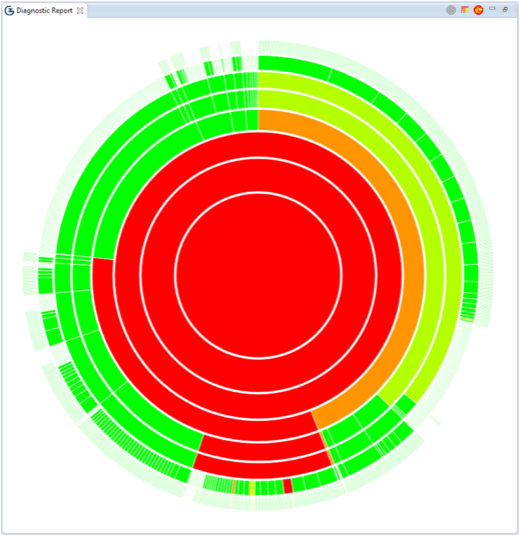
\includegraphics[width=0.5\textwidth]{barinel1.png}
    \caption{Sunburst visualization on Crowbar}
    \label{fig:crowbar-sunburst}
  \end{center}
\end{figure}

In addition to that information, this tool also shows us the component list sorted by fault likelihood.
%!TEX root = ../thesis.tex
\section{\emph{Software Repository Mining}}

\emph{Software Repository Mining} encompasses all \emph{software} which is able to extract data from repositories, such as \emph{Git} or \emph{SVN}.

\subsection{Corrections and defects identification}

While extracting information from code repositories, such as \emph{Git}, it is important to identify the types of changes that were made. A text description associated with the change is of the utmost importance for this identification, allowing it to be made with a high degree of precision, depending on the project \cite{Mockus2000}.

It is estimated that between 34 and 46\% of all changes are corrections and that they represent between 18 and 27\% of all added and removed lines of code \cite{Mockus2000}. There were also some patterns found relating code corrections with their size and with the day of the week in which they were executed \cite{Sliwerski2005}.

After this identification, it is possible to find out which changes have introduced the errors by using the \emph{SZZ} algorithm \cite{Sliwerski2005}. This algorithm analyzes the code and uses its history to correctly locate which \emph{commit} has introduced the defect, ignoring changes that only inserted comments, for example.

\subsection{Tools}

There are several tools to facilitate this process. Let us highlight two of them.

\subsubsection{\emph{libgit2}}

Libgit2\footnote{\url{https://libgit2.github.com/}} is a multi-platform library, without dependences, allowing a direct and native performance interaction with the \emph{Git} repository.

This library can be used with any language supporting \emph{C} bindings, so there are dozens of implementations using languages like \emph{Python}\footnote{pygit2 - \url{http://www.pygit2.org/}}, \emph{Javascript}\footnote{nodegit - \url{https://github.com/nodegit/nodegit}} and \emph{Java}\footnote{Jagged - \url{https://github.com/ethomson/jagged}}.

\subsubsection{\emph{GHTorrent}}

GHTorrent\footnote{\url{http://ghtorrent.org/}} is a project with the objective of creating a scalable and easily queriable (even \emph{offline}) database, which replicates the information obtained through the GitHub\footnote{\url{http://developer.github.com/}} REST API.

This tool works in a distributed way and monitors the GitHub API through the page \url{https://api.github.com/events}. Each event triggers an information and content extraction to a \emph{MongoDB} database and a different \emph{MySQL} database \cite{Gousios2012}.
%!TEX root = ../thesis.tex
\section{Approaches to defect prediction}

We have already explored some approaches to code quality prediction. In this chapter we will highlight some methods, like \emph{BugCache}, \emph{FixCache} and \emph{Buggy Change Classification}, which are included in the type of approach we want to follow (\emph{change log}) and that allow us, together with other methods, to optimize defect localization.

\subsection{\emph{BugCache/FixCache}}

Based on the assumption that faults never occur isolated, and therefore where there's a defect others can also exist, \emph{BugCache} creates a list of components which have a high probability of containing defects, based on an analysis of the complete changes history of the project.

This algorithm stands out due to its precision, managing a 73 to 95\% accuracy when used with file-level granularity, being the best to date \cite{kim2006automatic}.

Defects are identified by order of occurrence and added to the list. When that list reaches its maximum size, components start to be removed according to the chosen substitution method. There are several methods using different metrics, such as \emph{Least Recent Used - LRU}, number of recent defects and number of recent changes \cite{kim2006automatic}.

With this algorithm, we can conclude \cite{kim2006automatic}:
%
\begin{itemize}
	\item If a defect has been introduced, there is a tendency to soon introduce additional new defects (\emph{temporal locality})
	\item If a component was added or changed recently, it has a higher probability of defect (\emph{changed-entity locality}, \emph{new-entity locality})
	\item If a component has introduced an error, the components most directly connected to that one will also introduce errors in the future (\emph{spatial locality})
\end{itemize}

The difference between \emph{BugCache} and \emph{FixCache} is the time at which each one updates the list. The former updates the list when a defect is introduced, while the latter only updates when the error is fixed. Due to this difference, implementing \emph{FixCache} is easier.

\subsection{\emph{Buggy Change Classification}}

\emph{Change Classification} has a notably different approach and a very distinct objective too. \emph{Change Classification}, resorting to \emph{Machine Learning} methods and available information about previous errors, is able to predict if a change has introduced a new defect. This prediction has a high accuracy of 78\% \cite{Whitehead2008}.

In a first phase, all changes up to that moment are either classified as \emph{buggy} or \emph{clean}. After classifying them and extracting data for each one, a model is created by \"training\" a classification algorithm.

The types of data used are divided in seven groups: complexity metrics, added code, removed code, file and folder names, new code and meta-data \cite{Whitehead2008}.

Both \emph{Support Vector Machine} (SVM) and \emph{Naive Bayes} were used in the study, with the SVM-based classifier being the one with better results \cite{Whitehead2008}.

\subsection{Data-Augmented Software Diagnosis} \label{subsec:elmishali}

A different approach that also aims to help predict the location of software faults is Data-Augmented Software Diagnosis \cite{Elmishali}.

Model-based and spectrum-based approaches are able to identify faulty components with high precision and recall, but there is still room for improvement and since most projects use some kind of Version Control Software (VCS), there is a big amount of information that is not used. This opportunity is the foundation of the approach.

Barinel assumes that the defect probability, known as the prior, of every component is uniform, $0.001$. However, this approach proved it is possible to optimize Barinel results for Java projects by leveraging information about the project and supervised machine learning algorithms to predict the real component's defect probability.

First, healthy and faulty components are identified across the entire project's history according to Bug Trackers. For each component, a list of features, which is not specified, is extracted. The list is composed of traditional and object-oriented software complexity metrics, such as number of lines of code and cohesion, and values extracted from the software change history, like lines added or removed in last version and age of the file.

With the help of a supervised machine learning algorithm (either Random Forest, J48 or Naive Bayes) a model is created and used to classify each component in the project as healthy or faulty. The confidence that a component is faulty is then used as prior.

Experimental results revealed an increment both on precision and recall, see Figure \ref{fig:elmishali}. However, the solution was tested just on one project.
%
\begin{figure}%
    \centering
    \subfloat[Precision]{{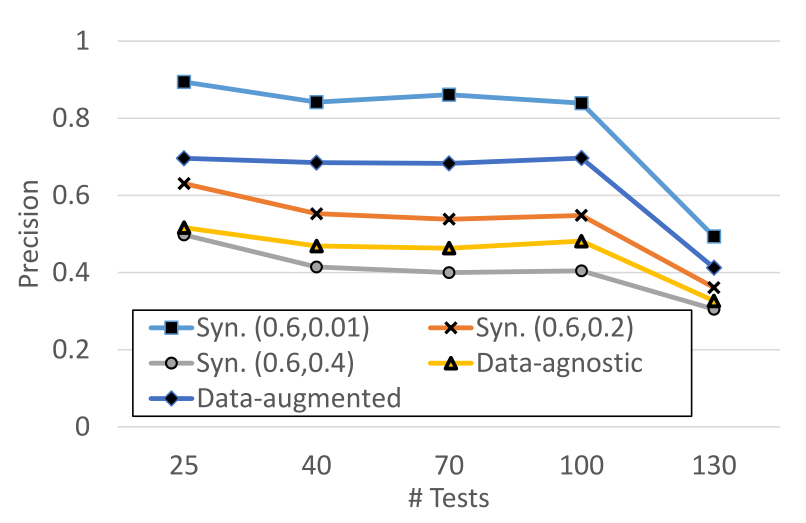
\includegraphics[width=0.4\textwidth]{elmishali-precision} }}%
    \qquad
    \subfloat[Recall]{{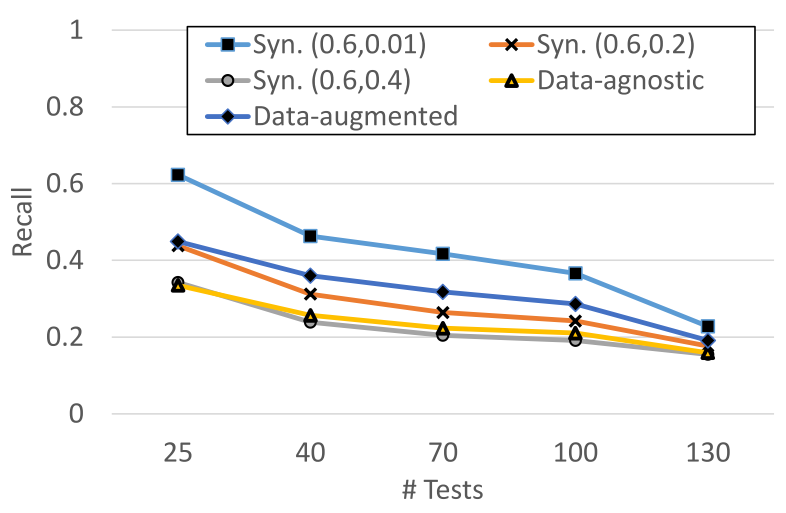
\includegraphics[width=0.4\textwidth]{elmishali-recall} }}%
    \caption{Diagnosis accuracy as a function of \# tests given to the diagnoser. \cite{Elmishali}}%
    \label{fig:elmishali}%
\end{figure}

\subsection{Time-weighted Risk}

Time-weighted risk is a formula developed at Google that helps in estimating component's reliability \cite{Lewis}. 
%
\begin{equation}
  \sum_{i=0}^{n}  \frac {1} {1 + e^{(-12 \cdot t_i) + W}}
\end{equation}

Where $i$ is a fixing commit, $t$ is the normalized change timestamp, from 0 to 1. If the change is at the start of the repository, the normalized timestamp will be 0. If instead the change is the last change made, the normalized timestamp will be 1. $W$ defines the weight of the decay, shifting the scoring curve along the x-axis.

The time-weighted curve produced by $\frac {1} {1 + e^{(-12 \cdot t_i) + W}}$ is the following:
%
\begin{figure}[H]
  \begin{center}
    \leavevmode
    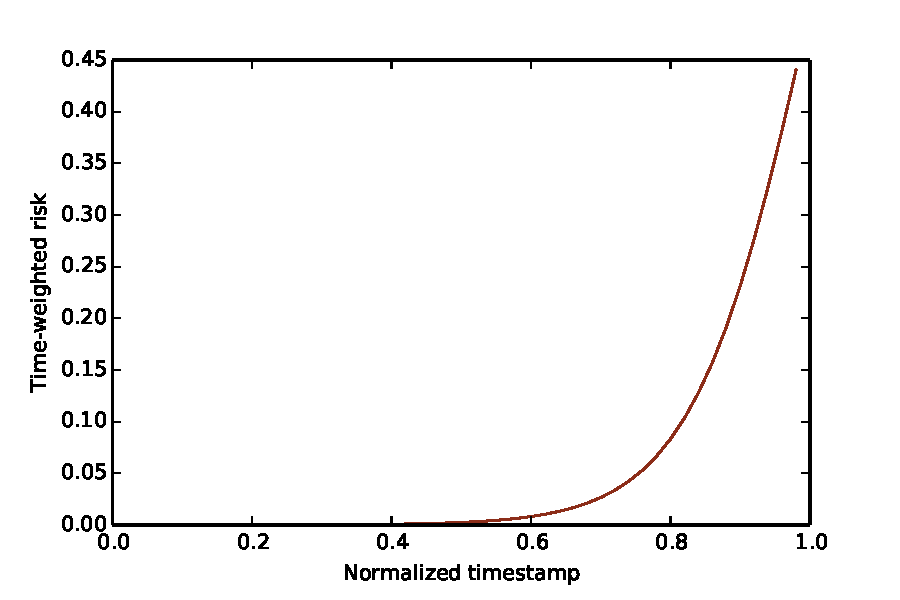
\includegraphics[width=0.5\textwidth]{twr.pdf}
    \caption{Time-weighted risk as function of the normalized timestamp of a given commit}
    \label{fig:crowbar-sunburst}
  \end{center}
\end{figure}

\todo{Talk about the Amir Elmishali's paper}

\todo{Add Background about Machine Learning?}